\documentclass[12pt]{article}
\usepackage{graphicx}
\usepackage {color}
\usepackage{pdfpages}
\usepackage{float}
\usepackage{changebar}
\usepackage{enumitem,amssymb}
\renewcommand{\familydefault}{\sfdefault}
\usepackage[margin=1.2in]{geometry}
\usepackage{graphicx}
\usepackage{wrapfig}
\usepackage[super]{cite}
\usepackage{subcaption}
\usepackage[table]{xcolor}
\usepackage{amsmath}
\usepackage[sort, numbers]{natbib}
\usepackage{multirow}
\usepackage{tabularx}
\usepackage{siunitx}
\usepackage{matlab-prettifier}
%%%%%%%%%%%%Defining the margins %%%%%%%%%%%%%%%%%%%%%
\textheight 9.in
\textwidth 6.5in
\topmargin -.5in
\oddsidemargin 0in
\setlength{\parskip}{\smallskipamount}

%%%%%%%%%%%%%%Specific Commands %%%%%%%%%%%%%%%%%%
\newcommand{\eg}{{\em e.g.,}}
\newcommand{\ie}{{\em i.e.,}}
\newcommand{\etc}{{\em etc.,}}
\newcommand{\etal}{{\em et al.}}
\newcommand{\degrees}{{$^{\circ}$}}
\newcommand{\fig}[1]{\textbf{Figure #1}}

%%%%%%%%%%%%%%%%%%%%%%%%%%%% Setting to control figure placement
% These determine the rules used to place floating objects like figures 
% They are only guides, but read the manual to see the effect of each.
\renewcommand{\topfraction}{.9}
\renewcommand{\bottomfraction}{.9}
\renewcommand{\textfraction}{.1}
\renewcommand{\familydefault}{\sfdefault} %setting the san serif font

%%%%%%%%%%%%%%%%%%%%%%%% Line spacing
% Use the following command for ``double'' spacing
%\setlength{\baselineskip}{1.2\baselineskip}
% and this one for an acceptable NIH spacing of 6lpi based on 11pt
%\setlength{\baselineskip}{.9\baselineskip}
% The baselineskip does not appear to work when we include a maketitle
% command in the main file.  Something there must set the line spacing
% If we use this next command, then things seem to work.
\renewcommand{\baselinestretch}{.9}

\setcounter{secnumdepth}{0} %make no numbers but have a table of contents


\begin{document}

\title{HW 1: Medical Imaging Systems}
\author{Jake Bergquist, u6010393 }
\maketitle

\section{Q1}\
\vspace{-.5in}
\subsection{a,b}
\begin{figure}[h]
	\centering
	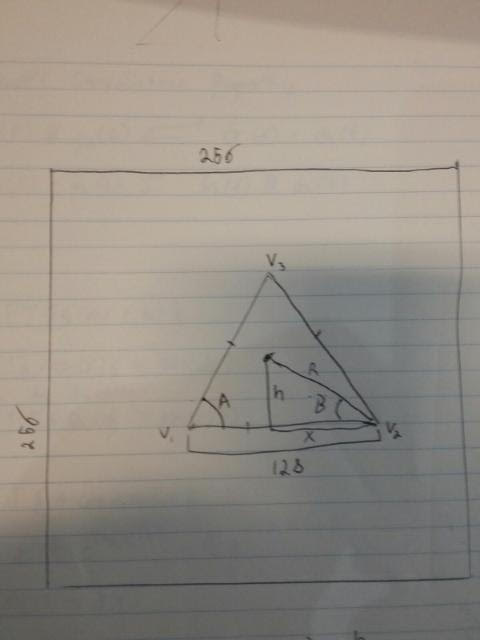
\includegraphics[width=0.5\textwidth]{Figures/drawnTriangle.png}
	\caption{Triangle within box drawn as instructed. The centroid of the triangle is at the centroid of the square. The sides of the triangle are 128 units. h denotes the distance from the centroid to the bottom side of the triangle. x denotes the bottom side of the smaller triangle fromed by h x and R. A is the angle of the larger triangle, at 60 \degrees. V1 V2 and V3 represent the vertexes of the triangle.}
	\label{Fig:Drawn_Triangle}
\end{figure}
When looking at Figure~\ref{Fig:Drawn_Triangle} we see the square with an equalateral triangle drawn in. The Sides of the square are 256, and the sides of the triangle are 160. The angle at each of the Vertices is A (60\degrees) and the distance from the centroid to the verticies is R. If we construct a sub triangle by making the line h from the centroid to the bottom side and using R we find a new angle B. This angle (B) is half of A (30\degrees).To find the location of the vertex V2 we need to calculate (Cx,Cy) + (x,-h) Where (Cx,Cy) are the coordinates of the center (128,-128). For V1 this would be (Cx,Cy) + (-x,-h), and for V3 it would be (Cx,Cy) + (0,R).Given the sub triangle we drew using R h and x we can calculate $x = 160/2$, $h = xTan(B)$ and $R = x/cos(B) =  h/sin(B)$

These verticie locations come out to be:

$x = 160/2 = 80$

$h = 46.1 -> 46$

$R = 92.3 -> 92$

$V1: (128,-128) + (-80,-46) = (48,-174)$

$V2: (128,-128) + (80,-46) = (208,-174)$

$V3 : (128,-128) + (0,92) = (128,-36)$

Now that we have the locations of the vertices we can calculate the lines that define these edges. We will use the slope intercept form.
For V1 to V2 the equation is $y = -174$.
For V1 to V3 the slope is $138/80$, the y intercept is $-256.8$, thus $y = (138/80)x - 256.8$
For V2 to V3 the slope is $-138/80$, the y intercept is $184.8$, thus $y = -(138/80)x + 184.8$
\subsection{c}
To define when a pixel is within the triangle it must be under V1 to V3 line, under the V3 to V2 line, and above the V1 to V2 line. To determine this we can take any point on the entire grid, and plug its x coordinate into one of the line formulas. This will produce a Y coordinate of the line of interest. If the y coordinate of our point is equal to the calculate y then our selected point is on the line. If the calculated y is greater than the point's y value the point is below the line, and if the calculated value is less than the point's y value then the point is above the line. In this way we can define the image mathematically. Because we are working with discrete numbers we will round the calculated value to the nearest integer.

Below is the MATLAB code used for problem1. In Figure~\ref{Fig:Matlab_Triangle} the resultant triangle drawn in a MATLAB figure is shown. The are within the triangle is set to a value of 1 and the area outside of the triangle is set to a value of 0.
\begin{lstlisting}[style=Matlab-editor]
%Problem 1
%Initilize matrices containing the x anbd y coordinates for each pixel
fig_yvals = zeros(256,256);
fig_xvals = fig_yvals;
for ind = 1:256
	fig_yvals(ind,:) = -ones(1,256)*ind;
	fig_xvals(:,ind) = ones(1,256)*ind;
end

%functions to define the lines defined at the end of the script
figTriangle = ((fig_yvals >= line1(fig_xvals)) +...
	       (fig_yvals <= line2(fig_xvals)) +...
	       (fig_yvals <= line3(fig_xvals))) == 3;

figure(1);
imshow(figTriangle);
title('Matlab Drawn Triangle')

function y = line1(x)
%v1 v2 line (line 1)
%y = -174
y = -174*ones(size(x));
end

function y = line2(x)
%v1 v3 line (line 2)
%y = (138/80)x - 256.8
y = (138/80).*x - 256.8;
end

function y = line3(x)
%v2 v3 line (line3)
%y = -(138/80)x + 184.8
y = -(138/80).*x + 184.8;
end
\end{lstlisting}




\begin{figure}[h]
	 \centering
	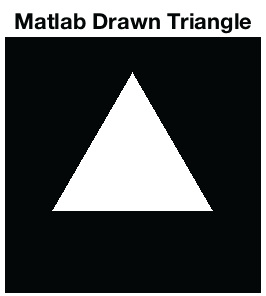
\includegraphics[width=0.5\textwidth]{Figures/matlabTriangle.png}
	\caption{The triangle drawn by the lines defined in the above matlab code. The box is 256 x 256 pixels. The triangle sides are 128 pixels in length and the triangle's center is at the center of the square.}
	\label{Fig:Matlab_Triangle}
\end{figure}


\section{Q2}\vspace{-.2in}
\subsection{a}

The code used to load and visualize the raw data magnitudes as a surface is shown below. As can be seen in Figure~\ref{Fig:freq_surf} there is a peak in the frequency spectrum near the center of the surface.
\begin{lstlisting}[style=Matlab-editor]
%plotblem 2

f_handle = fopen('Prob2.raw');%access the file location
raw_signal = fread(f_handle,[288,192],'float',0,'b');
%read in both the real and imaginary components at once
fclose(f_handle);
%Need to parse the input to be the complex matrix
raw_signal = [raw_signal(1:2:end,:)+raw_signal(2:2:end,:)*1i];
%Every second entry int he raw file is the previous entry's complex value

%Plotting the magintue of the signal as a surface
figure(1);clf();
surf((log(abs(raw_signal)))')
%during all visualizations the data is transposed
axis('equal')
axis('tight')
\end{lstlisting}


\begin{figure}[h]
	\centering
	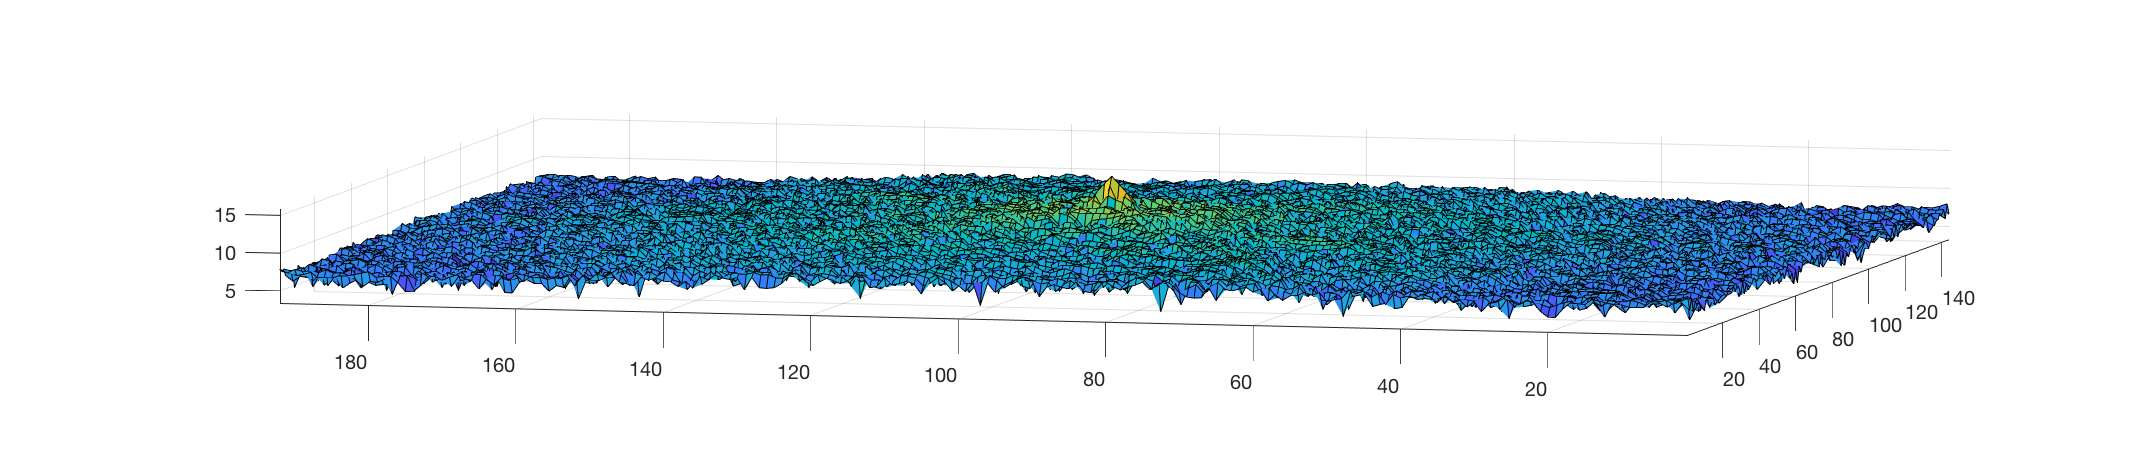
\includegraphics[width=\textwidth]{Figures/freqSurf.png}
	\caption{A surface representation of of the magnitudes of the raw signal data. As can be seen there is a peak at the center.}
	\label{Fig:freq_surf}
\end{figure}

\subsection{b}
The code to visualize as a 2D grayscale image is shown below. As can be seen in Figure~\ref{Fig:freq_img} there is a clear peak in magnitude at the center of the image. 
\begin{lstlisting}[style=Matlab-editor]
%%
%Showing the magnitude of the signal as grayscale
figure(2);clf()
imshow(rescale(log(abs(raw_signal)))');
axis('equal')
axis('tight')
\end{lstlisting}
\begin{figure}[h]
	\centering
	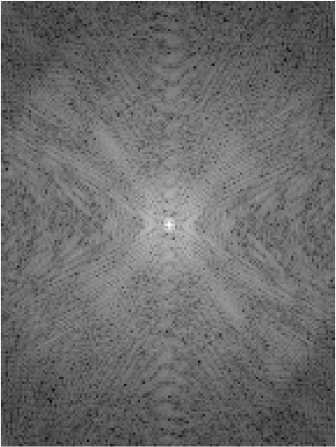
\includegraphics[width=.7\textwidth]{Figures/freqImg.png}
	\caption{An image showing the magnitudes of the raw signal encoded as grayscale value. Again it can be seen that there are large magnitudes at the center of the image.}
	\label{Fig:freq_img}
\end{figure}


\subsection{c,d}
The code for the forward and inverse reconstruction of the MRI image from the raw data is shown below. Figure~\ref{Fig:invFwd} shows the resultant reconstructions. At first glance the two look nearly identical. However the forward Fourier transform resulted in pixel intensity a few orders of magnitude higher than those of the inverse reconstruction. This is because of the sine difference between the inverse vs the forward transformation. This will also result in the second consequence which is that there will be a phase shift due to the change in sine.

\begin{lstlisting}[style=Matlab-editor]
%%
%reconstructing the image using inverse transform
MRI_Image = ifftshift(abs(ifft2(raw_signal)));

%Reconstructing using the forward transform
MRI_Image_Forward_FT = ifftshift(abs(fft2(raw_signal)));
figure(4);
subplot(121);
imagesc(MRI_Image')
axis('equal')
axis('tight')
title('Inverse Reconstruction')
colormap(gray);
subplot(122);
imagesc(MRI_Image')
axis('equal');
axis('tight')
title('Forward Reconstruction')
colormap(gray);

\end{lstlisting}
\begin{figure}[h]
	\centering
	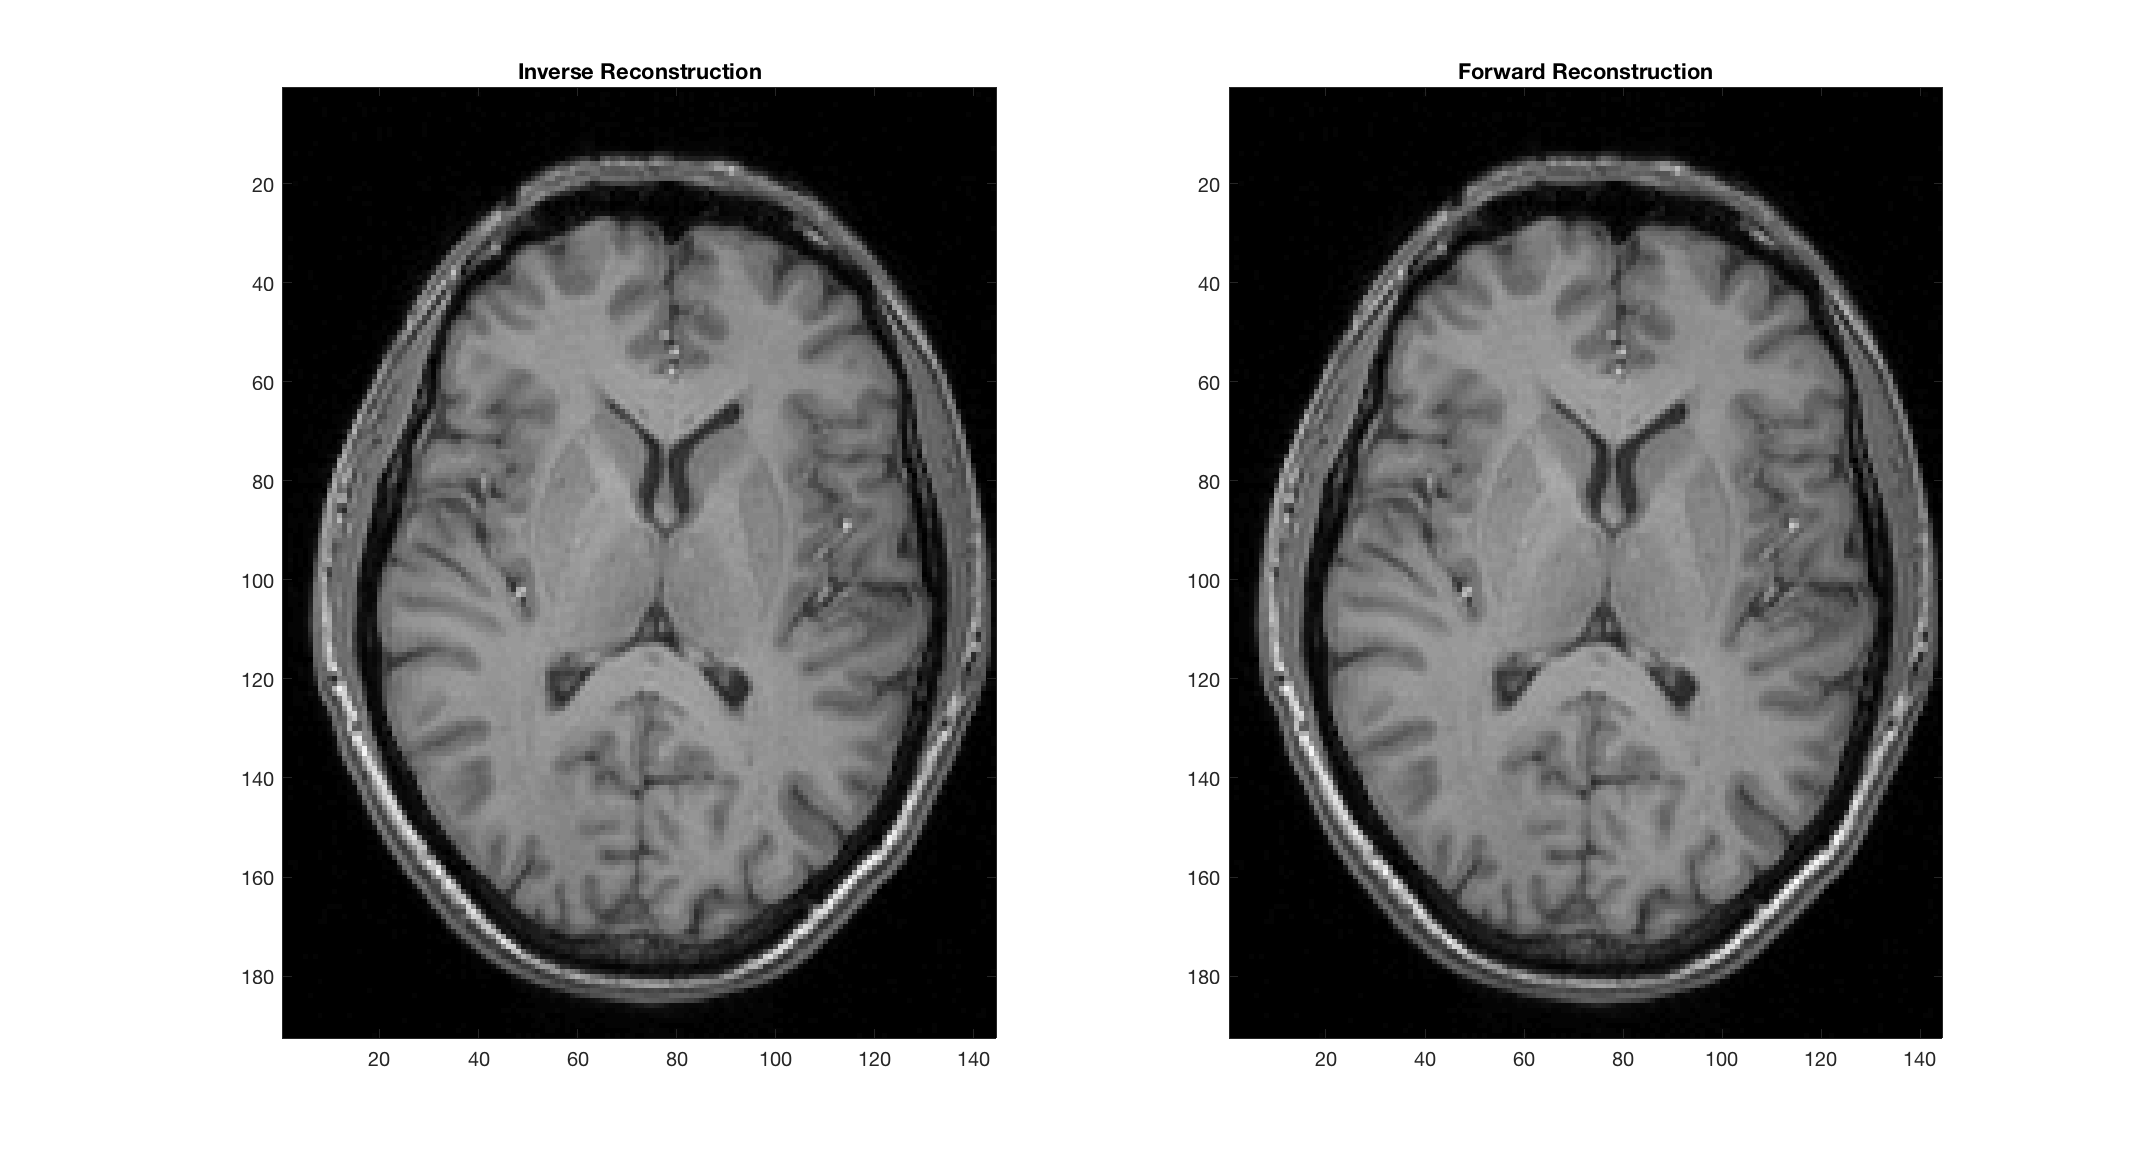
\includegraphics[width=\textwidth]{Figures/fwdVSinv.png}
	\caption{The reconstructed MRI images using inverse Fourier transform (left) and forward Fourier transform(right).}
	\label{Fig:invFwd}
\end{figure}
\vspace{-.3in}
\section{Q3}
In order to calculate the SNR I identified three regions of interest shown in Figure~\ref{Fig:segment} ashilighted by black boxes. These three regions were chosen in white matter across the brain. A section of background in the top corner was chosen to calculate the STD of the background of the image.(highlighted with a white box in Figure~\ref{Fig:segment}) The SNR measurements are summarized in Table~\ref{tab:snr}.
\begin{table}[H]
	\vspace{-.1in}
	\caption{\label{tab:snr} Numerical results from the SNR calculations.}
	\centering
	\begin{tabular}{|r|r|} \hline
		Region&SNR\\
		\hline
		R1&131.68\\
		R2&130.98\\
		R3&128.54\\
		Average&130.40\\
		\hline
		
		\hline
		
	\end{tabular}
\end{table}
\begin{figure}[h]
	\centering
	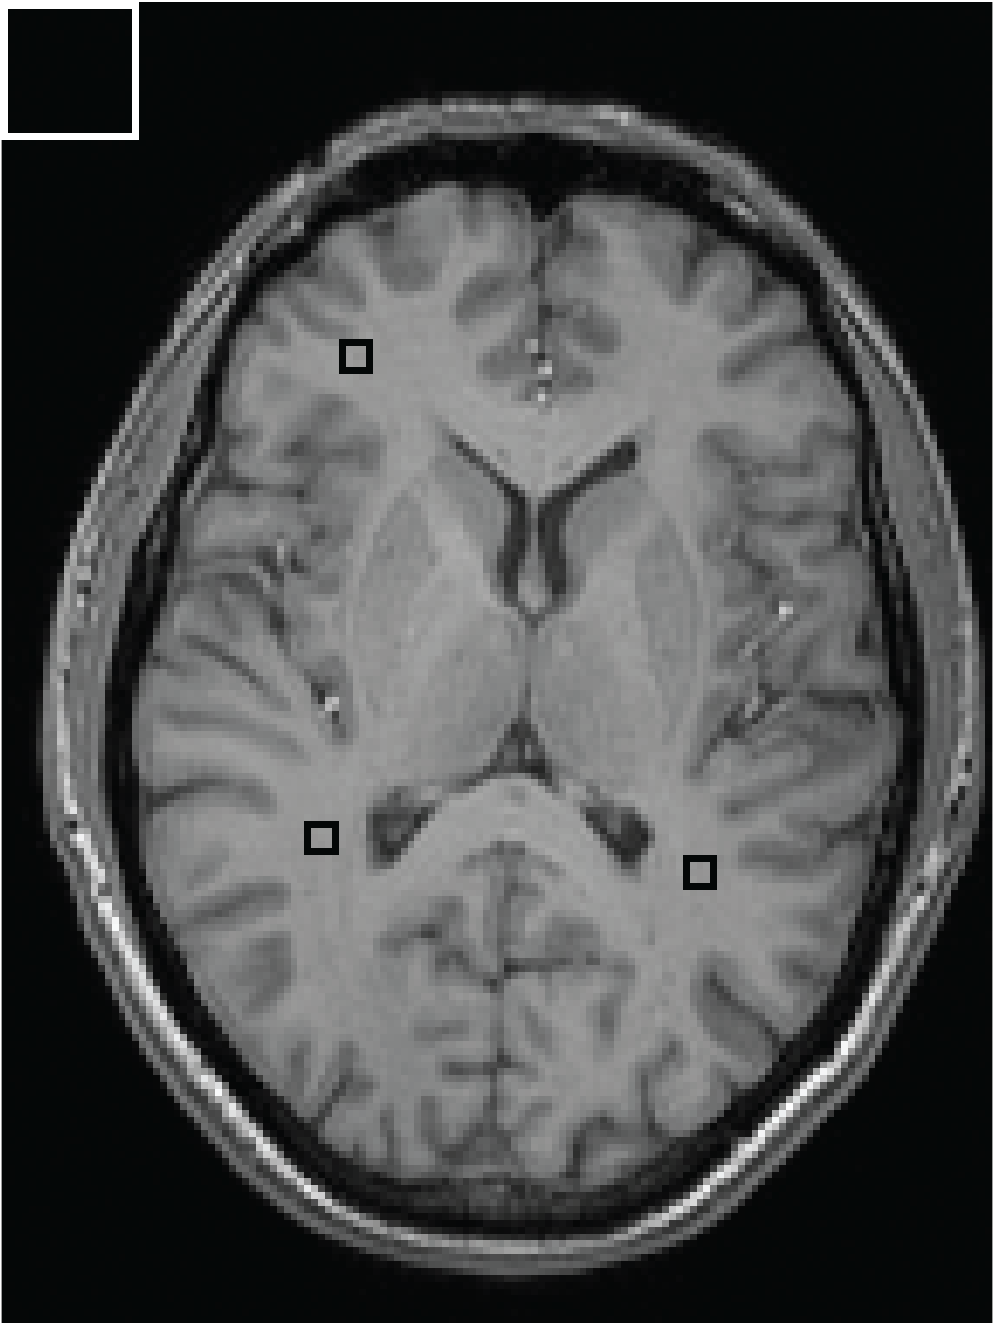
\includegraphics[width=.7\textwidth]{Figures/segment.png}
	\caption{The segmentations of the MRI image to use for SNR calculation are shown. The background area (top left) is highlighted with a white box. Region 1 (R1, top left), Region 2(R2, bottom left), and Region 3 (R3, bottom right) and hilighted with a black box. The regions of interests include the box that highlights them.}
	\label{Fig:segment}
\end{figure}



\begin{lstlisting}[style=Matlab-editor]
%%
%selecting background section. We will grab a section of the background
%outside of the head in the top corner near the origin. The first 20 x 20
%patch of any of the corners will do

background = MRI_Image(1:20,1:20);
backgroundSegment = Segmented_MRI(1:20,1:20);%For vis purposes
Segmented_MRI(1:20,1:20) = 255;%Outline the backgound ROI
Segmented_MRI(2:19,2:19) = backgroundSegment(2:19,2:19);

%three regions of interest are chosen from the white matter
r1_coords = [50,50,54,54];
r1_vals = MRI_Image(r1_coords(1):r1_coords(3),...
		    r1_coords(2):r1_coords(4));
r1_vals_segment = Segmented_MRI(r1_coords(1):r1_coords(3),...
				r1_coords(2):r1_coords(4));
				%For vis purposes
Segmented_MRI(r1_coords(1):r1_coords(3),...
	      r1_coords(2):r1_coords(4),1) = 0;%Color the ROI Black
%replace the center to make a black box outlining the ROI
Segmented_MRI(r1_coords(1)+1:r1_coords(3)-1,r1_coords(2)+1:r1_coords(4)-1) = r1_vals_segment(2:end-1,2:end-1);



r2_coords =[45,120,49,124];
r2_vals = MRI_Image(r2_coords(1):r2_coords(3),...
		    r2_coords(2):r2_coords(4));
r2_vals_segment = Segmented_MRI(r2_coords(1):r2_coords(3),...
		  	        r2_coords(2):r2_coords(4));
		  	        %For vis purposes
Segmented_MRI(r2_coords(1):r2_coords(3),...
      	      r2_coords(2):r2_coords(4),1) = 0;%Color the ROI Black
%replace the center to make a black box outlining the ROI
Segmented_MRI(r2_coords(1)+1:r2_coords(3)-1,r2_coords(2)+1:r2_coords(4)-1) = r2_vals_segment(2:end-1,2:end-1);

r3_coords =[100,125,104,129];
r3_vals = MRI_Image(r3_coords(1):r3_coords(3),...
		    r3_coords(2):r3_coords(4));
r3_vals_segment = Segmented_MRI(r3_coords(1):r3_coords(3),...
		      		r3_coords(2):r3_coords(4));
		      		%For vis purposes
Segmented_MRI(r3_coords(1):r3_coords(3),...
              r3_coords(2):r3_coords(4),1) = 0;%Color the ROI Black
%replace the center to make a black box outlining the ROI
Segmented_MRI(r3_coords(1)+1:r3_coords(3)-1,r3_coords(2)+1:r3_coords(4)-1) = r3_vals_segment(2:end-1,2:end-1);
figure(1);
imshow(Segmented_MRI');
axis('equal')
axis('tight')
%Calculate SNR
background_STD = std2(background);

snr_1 = mean(r1_vals(:))/background_STD;
snr_2 = mean(r2_vals(:))/background_STD;
snr_3 = mean(r3_vals(:))/background_STD;
mean_snr = mean([snr_1,snr_2,snr_3]);
\end{lstlisting}
\vspace{-.3in}
\section{Q4}
The results of the sub-sampling of the raw signal are shown in Figure~\ref{Fig:subset}. As can be seen, only using the central 50\% of the signal results in a reconstruction that still shows the major anatomical components but appears blurred and grainy. This is because we have omitted the high frequency components of the image which results in a blurry/sub sampled image. In the second sub sampling example when we only take every other entry from the raw data we are left witht he reconstruction seen in Figure~\ref{Fig:subset} on the right. This image is grainer as well as badly aliased. This makes sens if we consider that we have sampled our signal int he frequency domain at a resolution that is insufficient to properly reconstruct the signal. 

\begin{figure}[H]

	\centering
	
	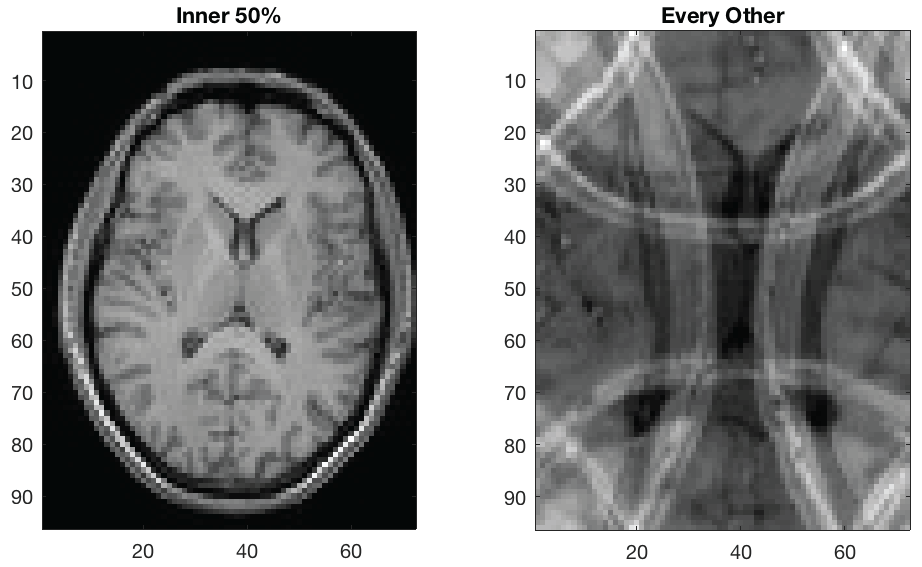
\includegraphics[width=.8\textwidth]{Figures/subset.png}
		
	\caption{The wo reconstructions using a subset of the raw signal data. On the left the reconstruction using the inner 50\% of the data shows a more grainy and lower resolution image. The right shows the result of using every other entry of the raw signal which shows aliasing as well as lower resolution.}
	\label{Fig:subset}
\end{figure}
\begin{lstlisting}[style=Matlab-editor]

%%
%problem 4
%The center 50% would be the center 72x96
center_raw = raw_signal(37:36+72,49:48+96);
MRI_Image_center_subset = ifftshift(abs(ifft2(center_raw)));

everyOther_raw = raw_signal(1:2:end,1:2:end);
MRI_Image_everyOther_subset = ifftshift(abs(ifft2(everyOther_raw)));

figure(1);
subplot(121);
imagesc(MRI_Image_center_subset')
axis('equal')
axis('tight')
title('Inner 50%');
colormap(gray);
subplot(122);
imagesc(MRI_Image_everyOther_subset')
axis('equal');
axis('tight')
title('Every Other');
colormap(gray);

\end{lstlisting}


\section{Q5}

The three kernels presented are very common. Kernel a is a 3x3 averaging filter that will smooth an image by averaging every pixel value to be the mean of itself and its 8 connected neighbors. Kernel b is an edge detection kernel/derivative kernel for the y direction. This kernel will respond at areas of high derivative along the y axis. Positive derivatives will result in a  positive response and negative derivatives will result in a negative response in the y direction. The c filter is just like b but for the x axis. These results can be seen in Figure~\ref{Fig:conv}. The first panel on the top left shows the original image. The second panel on the top right shows the convolution with the 3x3 averaging filter, a smoothed version of the original image where lines have been blurred. The next two panels show the convolutions with the two edge/derivative filters. On the bottom left is the vertical edge detector that shows positive response when the signal transitions from low intensity to high at an edge and negative response when the intensity transitions from high to low. This results in the outlines of the structures as scanned from the vertical axis being accentuated. The same kind of effect is seen int he bottom right panel for kernel c, the horizontal derivative/edge filter. These two filters combined can help draw outlines around the various structures in the image and allow for some level of automatic segmentation. Notice how the vertical edge detector has little to no response for vertical lines, this is because by 'vertical edge detector' I mean that it is scanning the vertical (y) axis, detecting horizontal lines. The same logic is true for the last kernel that scans the horizontal axis looking for vertical lines.

The code to perform these convolutions is shown below the figure.

\begin{figure}[H]
	\centering
	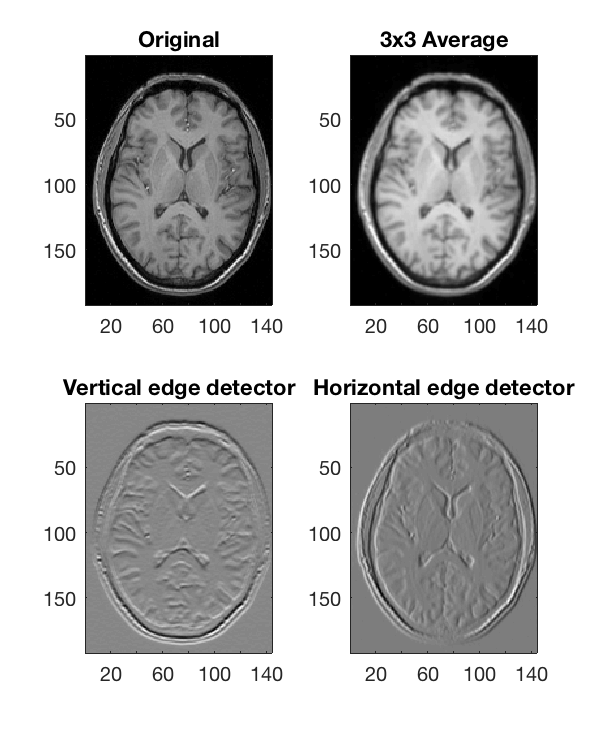
\includegraphics[width=\textwidth]{Figures/convs.png}
	\caption{}
	\label{Fig:conv}
\end{figure}
\begin{lstlisting}[style=Matlab-editor]
%%
%Problem 5

%kernal a
averaging_kernal = ones(3,3)/9;

%kernal b
%orientation flipped due to matlab conventions
vertical_edge_detector = zeros(3,3);
vertical_edge_detector(:,3) = 1;
vertical_edge_detector(:,1) = -1;

%kernal c
%orientation flipped due to matlab conventions
horizontal_edge_detector = zeros(3,3);
horizontal_edge_detector(1,:) = 1;
horizontal_edge_detector(3,:) = -1;

conv1_results = ...
conv2(MRI_Image,averaging_kernal,'same');
%I use the same argument to not get increased image size
%It does however leave in zero padded edges in the calculation but the
%edges are all background and I do not mind as much there

conv2_results = ...
conv2(MRI_Image,vertical_edge_detector,'same');

conv3_results = ...
conv2(MRI_Image,horizontal_edge_detector,'same');

figure(1);
subplot(2,2,1);
imagesc(MRI_Image')
axis('equal')
axis('tight')
colormap(gray);
title('Original')
subplot(222);
imagesc(conv1_results')
axis('equal')
axis('tight')
colormap(gray);
title('3x3 Average')
subplot(223);
imagesc(conv2_results')
axis('equal')
axis('tight')
colormap(gray);
title('Vertical edge detector')
subplot(224);
imagesc(conv3_results')
axis('equal')
axis('tight')
colormap(gray);
title('Horizontal edge detector')

\end{lstlisting}

%%%%%%%%%%%%%%%%%% Correct Bibliography Style




\end{document}








